\documentclass[12pt,letterpaper]{article}

\usepackage[margin=1in]{geometry}
\usepackage{setspace}
\usepackage{iftex}

\ifPDFTeX
  \usepackage[T1]{fontenc}
  \usepackage[utf8]{inputenc}
  \usepackage{newtxtext,newtxmath}
\else
  \usepackage{fontspec}
  \setmainfont{Times New Roman}
\fi

\usepackage{amsmath}
\usepackage{amssymb}
\usepackage{booktabs}
\usepackage{graphicx}
\usepackage{hyperref}
\usepackage[version=4]{mhchem}
\usepackage{siunitx}
\usepackage{subcaption}

\hypersetup{
  colorlinks = false,
  pdfauthor = {Rees Verleur},
  pdftitle = {ME 617 Mock Lab Report}
}

\singlespacing

\title{ME 617 Mock Lab Report}
\author{Rees Verleur}
\date{\today}

\begin{document}

\maketitle

\section{Introduction and Objectives}

This mock lab uses scanned-wavelength absorption spectroscopy to recover temperature, pressure, and CO mole fraction in shocked gas. The data set contains a baseline scan, an etalon scan for time-to-wavenumber calibration, and repeated shock-tube scans across a CO feature group near \SI{2008.5}{\per\centi\meter}. The reduction converts detector voltage to absorbance for each laser sweep, fits the resulting spectrum with a constrained three-line Voigt model, and reconstructs the gas state as a function of time.

The measurement couples a shock tube with a non-intrusive quantum cascade laser diagnostic. The overall workflow follows the same measurement logic as Mathews et al. [1], but is applied here to the provided course data and to the simplified modeling choices adopted for this report. The objective is to obtain scan-resolved temperature, pressure, and \ce{CO} mole fraction, then quantify the uncertainty associated with those estimates.

\section{Theory}

\subsection*{Shock-Tube Context}

A shock tube produces an abrupt rise in gas temperature and pressure by separating a high-pressure driver gas from a lower-pressure driven gas with a diaphragm. After rupture, an incident shock propagates into the driven section and creates the compressed state known as Region 2. Reflection from the end wall further compresses and heats the gas while reducing the bulk velocity to nearly zero; the reflected-shock state is Region 5. Region 5 is usually the target state for shock-tube spectroscopy because it is hotter, denser, and closer to spatially uniform over the observation time of interest.

Because the state change occurs over a very short time scale, shock tubes provide a well-defined starting point for high-temperature measurements. The optical section is therefore placed near the end wall to minimize the delay between incident- and reflected-shock arrival while avoiding the strongest end-wall disturbances. In this experiment, the measured CO absorption is used to recover scan-resolved temperature, pressure, and CO mole fraction through the shocked-gas event.

\subsection*{Absorbance and Beer--Lambert Law}
The starting point for direct absorption spectroscopy is the one-dimensional radiative-transfer equation. For a non-scattering medium,

\begin{equation}
  \frac{dI_{\tilde{\nu}}}{dx}
  =
  k_{\tilde{\nu}}\left(I_{\tilde{\nu}}^{\mathrm{bb}} - I_{\tilde{\nu}}\right)
\end{equation}

where $I_{\tilde{\nu}}$ is the spectral intensity at wavenumber $\tilde{\nu}$, $I_{\tilde{\nu}}^{\mathrm{bb}}$ is the blackbody intensity, and $k_{\tilde{\nu}}$ is the spectral absorption coefficient in cm$^{-1}$. If the path is uniform, integration over a path length $L$ gives

\begin{equation}
  I_{\tilde{\nu}}(L)
  =
  I_{\tilde{\nu},0}\exp(-k_{\tilde{\nu}}L)
  +
  I_{\tilde{\nu}}^{\mathrm{bb}}\left[1-\exp(-k_{\tilde{\nu}}L)\right]
\end{equation}

For the present measurements, laser intensity is much larger than gas self-emission, so the emission term is neglected. The transmitted intensity then reduces to the Beer--Lambert form,

\begin{equation}
  I_{\tilde{\nu}}(L)
  =
  I_{\tilde{\nu},0}\exp(-\kappa_{\tilde{\nu}}L)
\end{equation}

Under the independent-line approximation, the absorption coefficient is written as

\begin{equation}
  \kappa_{\tilde{\nu}}
  =
  \sum_i \kappa_{\tilde{\nu},i}
  =
  PX\sum_i S_i(T)\phi_i(\tilde{\nu})
\end{equation}

where $P$ is pressure in atm, $X$ is absorber mole fraction, $S_i(T)$ is the line strength in cm$^{-2}$/atm, and $\phi_i(\tilde{\nu})$ is a normalized line-shape function in cm. The absorbance model used throughout the analysis is therefore

\begin{equation}
  \alpha(\tilde{\nu})
  =
  \kappa_{\tilde{\nu}}L
  =
  PXL\sum_i S_i(T)\phi_i(\tilde{\nu})
\end{equation}

For a normalized line shape, the integrated absorbance area of line $i$ is $PXL\,S_i(T)$.

\subsection*{Temperature-Dependent Line Strength}

The line strength $S_i(T)$ is the integrated absorption strength of transition $i$. Reference values are taken from HiTEMP at a standard temperature $T_0$ and scaled to the local gas temperature with the standard HITRAN/HiTEMP correction,

\begin{equation}
  S_i(T)=S_i(T_0)\frac{Q(T_0)}{Q(T)}\frac{T_0}{T}
  \exp\!\left[-\frac{hcE_i''}{k_B}\!\left(\frac{1}{T}-\frac{1}{T_0}\right)\right]
  \frac{1-\exp\!\left(-\frac{hc\tilde{\nu}_{0,i}}{k_B T}\right)}{1-\exp\!\left(-\frac{hc\tilde{\nu}_{0,i}}{k_B T_0}\right)}
\end{equation}

Here $Q(T)$ is the molecular partition sum, $E_i''$ is the lower-state energy, and $\tilde{\nu}_{0,i}$ is the line center. The correction accounts for the changing partition function, Boltzmann population of the lower state, and stimulated emission. Differences in $S_i(T)$ among nearby transitions provide part of the temperature sensitivity of the measured spectrum.

\subsection*{Line Shapes and Collisional Broadening}

The line-shape function $\phi_i(\tilde{\nu})$ distributes the integrated line strength about the line center. For the present spectra, the important broadening mechanisms are Doppler broadening from thermal molecular motion and collisional broadening from intermolecular collisions. Natural broadening is negligible and is omitted.

Doppler broadening produces a Gaussian contribution, while collisional broadening produces a Lorentzian contribution. When both are important, the line shape is well represented by a Voigt profile. For transition $i$,

\begin{equation}
  \phi_i(\tilde{\nu})
  =
  \phi_{V,i}\!\left[\tilde{\nu}-\tilde{\nu}_{0,i};\,\Delta\tilde{\nu}_{D,i},\,\Delta\tilde{\nu}_{C,i}\right]
\end{equation}

where $\Delta\tilde{\nu}_{D,i}$ and $\Delta\tilde{\nu}_{C,i}$ are the Doppler and collisional full widths at half maximum. The Doppler width follows from kinetic theory,

\begin{equation}
  \Delta\tilde{\nu}_{D,i}
  =
  2\tilde{\nu}_{0,i}
  \sqrt{\frac{2k_B T \ln 2}{mc^2}}
\end{equation}

The collisional width depends on pressure and on the broadening properties of the collision partners. If the tabulated coefficients are given as Lorentz half-widths $\gamma_{k,i,\mathrm{ref}}$, the corresponding collisional FWHM is

\begin{equation}
  \Delta\tilde{\nu}_{C,i}(T)
  =
  2P\sum_k X_k\,\gamma_{k,i,\mathrm{ref}}
  \left(\frac{T_{\mathrm{ref}}}{T}\right)^{n_{k,i}}
\end{equation}

where $X_k$ is the mole fraction of collision partner $k$ and $n_{k,i}$ is the corresponding temperature exponent. In this problem, the Doppler contribution carries most of the direct temperature sensitivity, while the collisional contribution carries most of the direct pressure sensitivity.

\section{Experimental Setup and Procedure}

\subsection*{Shock-Tube and Optical Setup}

Measurements were acquired in Purdue's High-Pressure Shock Tube. The driven gas was 2\% CO, 1.8\% \ce{CO2}, and balance \ce{N2}. After diaphragm rupture, the incident shock produced Region 2 and reflection from the end wall produced Region 5 at the optical test section. The handout target for Region 5 was approximately \SI{4000}{K} and \SI{1}{atm}. The shock-tube internal diameter, and therefore the absorption path length used here, was \SI{10.32}{cm}.

A quantum cascade laser near \SI{4.98}{\micro\meter} scanned the CO feature group by current modulation. The applied modulation was \SIrange{0}{620}{mV} at \SI{300}{kHz}, giving one sweep every \SI{3.33}{\micro\second}. Because QCL tuning is partly thermal, the frequency sweep is only approximately repeatable from scan to scan, so a separate frequency calibration is required. The transmitted beam was measured with a detector whose voltage output was taken to be linear in incident optical intensity.

\subsection*{Measurement Procedure and Calibration Data}

The analysis uses three provided datasets: a baseline scan with no absorbing gas in the beam path, an etalon scan, and the shock-tube measurement. Each file also contains a TTL reference from the function generator, which is used to align the repeated sweeps. The baseline data define the unabsorbed transmission, and the shocked-gas transmission is compared against that baseline to obtain absorbance.

The etalon measurement determines how laser frequency changes during each sweep. A solid germanium Fabry--Perot etalon, 3 in. long, was placed in the beam path. Interference between the transmitted and reflected beams produces periodic maxima as the wavelength is scanned. The spacing between adjacent maxima is the free spectral range,

\begin{equation}
  \mathrm{FSR} = \frac{1}{2nL}
  \approx
  \SI{0.0163}{\per\centi\meter},
\end{equation}

where $L = \SI{7.62}{cm}$ and the refractive index of germanium at this wavelength is $n = 4.019$. This periodic reference provides the time-to-wavenumber calibration used for the shock and baseline scans.

\subsection*{Scanned CO Transitions}

The scan window covered the three CO transitions listed below.

\begin{table}[h]
  \centering
  \footnotesize
  \setlength{\tabcolsep}{5pt}
  \caption{Spectroscopic parameters for the scanned CO transitions.}
  \label{tab:co-transitions}
  \resizebox{\textwidth}{!}{%
    \begin{tabular}{lccccccc}
      \toprule
      Transition & $\tilde{\nu}_0$ & $S_{\mathrm{ref}}(T_0 = 296\,\mathrm{K})$ & $E''$ & $\gamma_{\ce{CO}-\ce{N2}}$ & $n_{\ce{N2}}$ & $\gamma_{\ce{CO}-\ce{CO}}$ & $n_{\ce{CO}}$ \\
      & [cm$^{-1}$] & [cm$^{-1}$/(\mbox{molec-cm}$^{-2}$)] & [cm$^{-1}$] & [cm$^{-1}$/atm] & [-] & [cm$^{-1}$/atm] & [-] \\
      \midrule
      P(0,31) & 2008.525 & 2.669e-22 & 1901.131 & 0.0412 & 0.47 & 0.0430 & 0.5 \\
      P(2,20) & 2008.422 & 1.149e-28 & 5051.740 & 0.0526 & 0.57 & 0.0550 & 0.5 \\
      P(3,14) & 2008.552 & 2.877e-32 & 6742.874 & 0.0607 & 0.65 & 0.0610 & 0.5 \\
      \bottomrule
    \end{tabular}%
  }
\end{table}

These three transitions are a useful set because they fall within a single QCL scan window but span large differences in line strength and lower-state energy, so the combined spectrum carries temperature sensitivity through the relative peak strengths and pressure/composition sensitivity through the line area and collisional broadening.

\section{Data Reduction}

\subsection*{Signal Loading and Sweep Extraction}

Each MAT file contains a detector channel and a TTL-like reference channel from the function generator. The reference signal is thresholded to identify sweep boundaries, and the sample period is inferred from the known \SI{300}{kHz} modulation frequency. The continuous records are then split into individual sweeps on a common local time axis. A fixed phase offset of \SI{2.2}{\micro\second} is applied before the trace is reshaped so that the first incomplete sweep is discarded and each retained sweep begins with a short section of baseline, spans the useful laser ramp, and ends with a small amount of trailing baseline. This sacrifices a small amount of edge data, but it gives a consistent registration across the baseline, etalon, and shock datasets.

\subsection*{Baseline Treatment and Absorbance Construction}

The baseline sweeps are first registered as described above and then averaged to form a single reference sweep. Because the absorbance calculation assumes that the detector voltage is linear in optical intensity, Beer--Lambert absorbance can be evaluated directly from the voltage ratio,
\[
  A = -\ln\!\left(I/I_0\right),
\]
where $I_0$ is the baseline signal and $I$ is the shocked-gas transmission. Before this ratio is formed, a linear wing baseline is fit through the flat regions at the beginning and end of each sweep and subtracted. The same correction is applied to the average baseline sweep and to every shock sweep. This removes slow scan-to-scan intensity drift and any small broadband slope within a single sweep that would otherwise appear as artificial absorbance. After line correction, each shock sweep is scaled so that its peak matches the peak of the corrected average baseline. This makes the absorbance construction less sensitive to overall amplitude variation between scans while preserving the within-scan absorption features.

Absorbance is evaluated only over the part of the ramp where the corrected average baseline lies between about \SI{1.0}{V} and \SI{2.75}{V}. The lower cutoff removes the low-signal beginning of the scan, where the transmission ratio is noisy and the signal-to-noise ratio is poor. The upper cutoff avoids the highest-voltage end of the ramp near the scan maximum, where the sweep is less useful for the present analysis. Samples with non-positive transmission ratios are excluded because Beer--Lambert absorbance is undefined there.

A representative time-domain reduction is shown in Fig.~\ref{fig:shock-time}. The left panel compares the corrected average baseline with one corrected shock sweep. Outside the absorbing portions of the scan the two traces nearly coincide, while the departures between them mark the CO absorption features. The right panel shows the corresponding absorbance in the retained part of the sweep before conversion to frequency.

\begin{figure}[tbp]
  \centering
  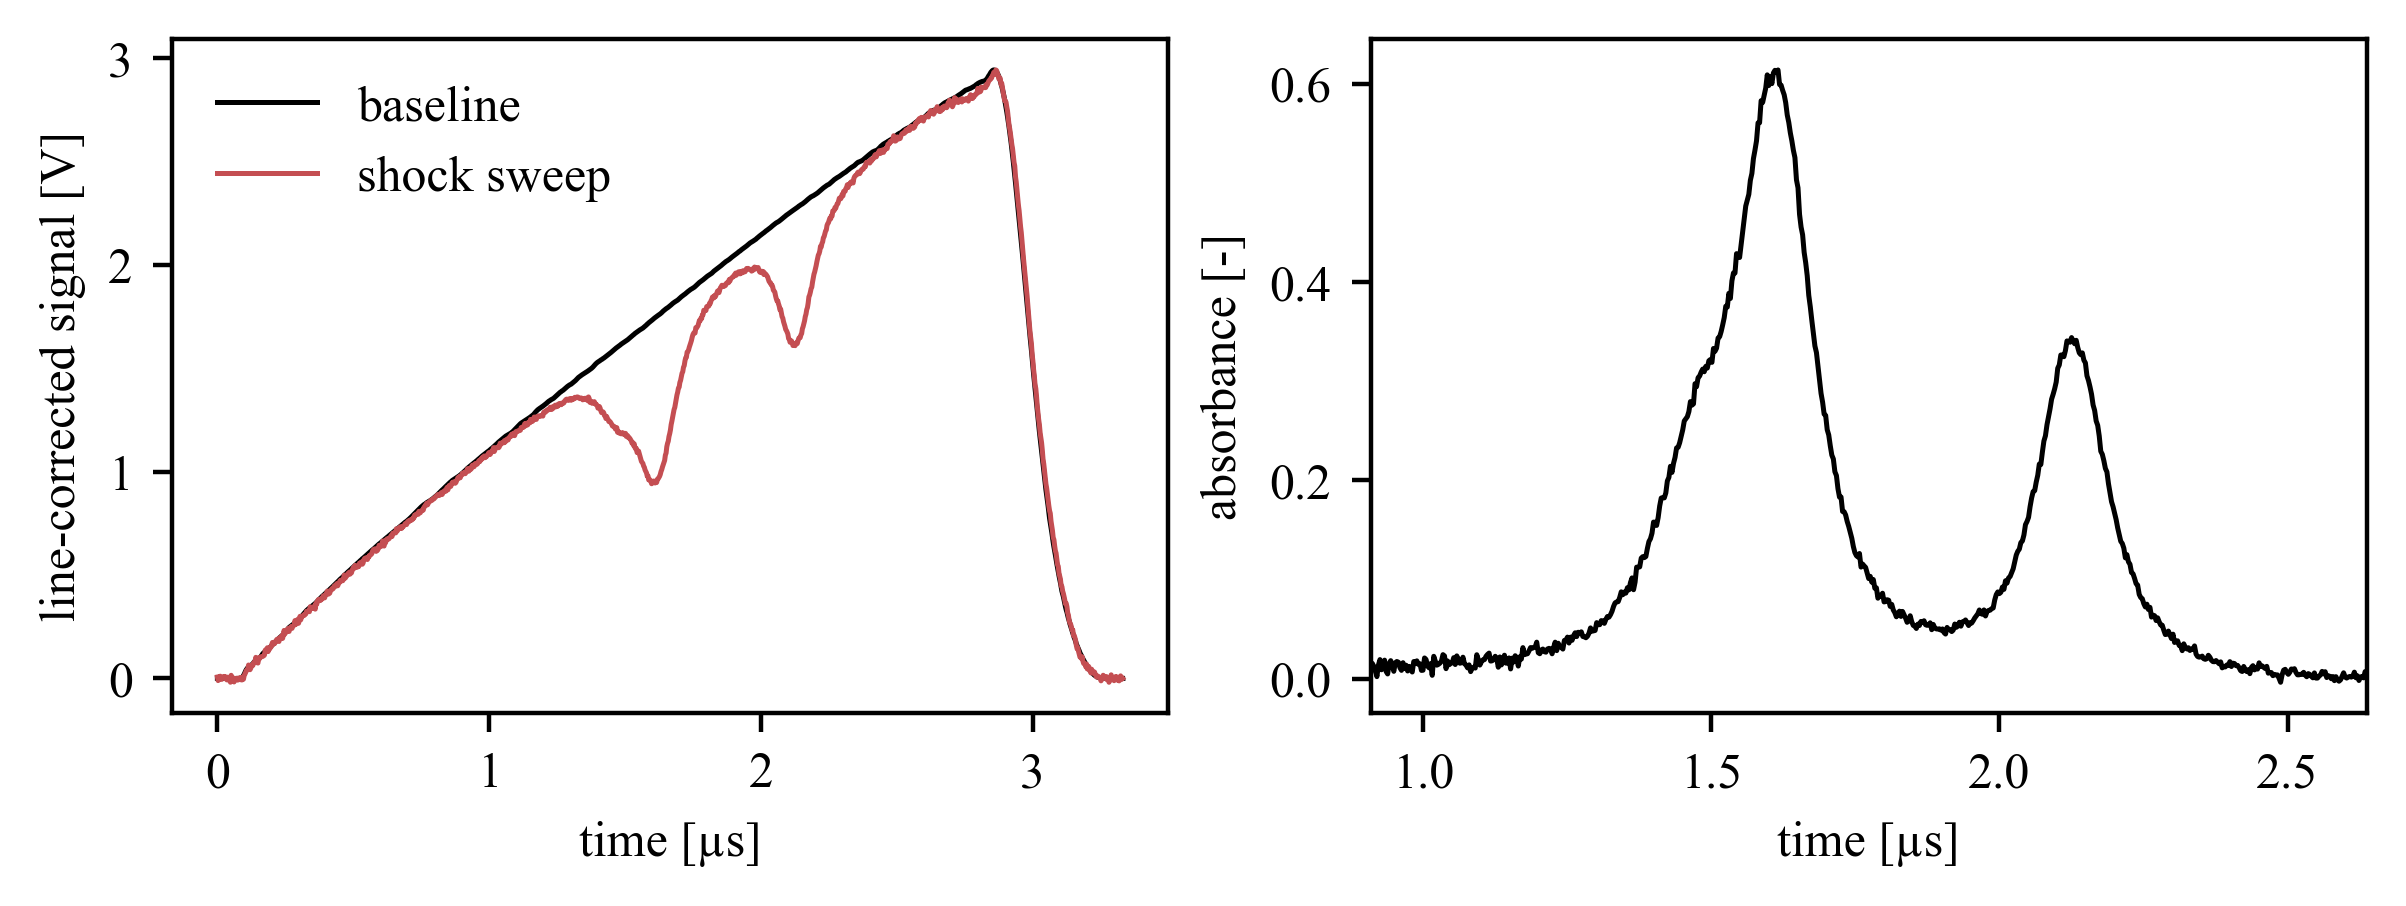
\includegraphics[width=\linewidth]{figures/shock_time.png}
  \caption{Representative time-domain reduction. Left: corrected average baseline and one corrected shock sweep. Right: absorbance computed from the retained time window of that sweep.}
  \label{fig:shock-time}
\end{figure}

\subsection*{Etalon Calibration}

The etalon data are used to convert sweep time to relative wavenumber. Each etalon sweep is first baseline-corrected using its edge samples so that the fringe extrema can be identified cleanly. Fringe peaks are then detected on the registered scans, the peak locations are averaged by fringe order, and those averaged peak times are assigned equally spaced relative wavenumbers using the known germanium etalon free spectral range. The final time-to-wavenumber relation is represented by a quartic polynomial,

\begin{equation}
  \Delta\tilde{\nu}(t)=a_0+a_1 t+a_2 t^2+a_3 t^3+a_4 t^4,
\end{equation}

which is sufficient to capture the modest nonlinearity in the QCL frequency sweep. This calibration is relative rather than absolute: it defines a consistent wavenumber axis within the scan window, but it does not lock the spectrum to an external absolute frequency standard.

The etalon calibration is shown in Fig.~\ref{fig:etalon-cal}. The left panel shows a representative corrected etalon sweep with the detected fringe peaks. The right panel shows the quartic time-to-wavenumber fit and its residuals. The residuals remain small compared with the etalon free spectral range, so the quartic is adequate over the useful scan interval.

\begin{figure}[tbp]
  \centering
  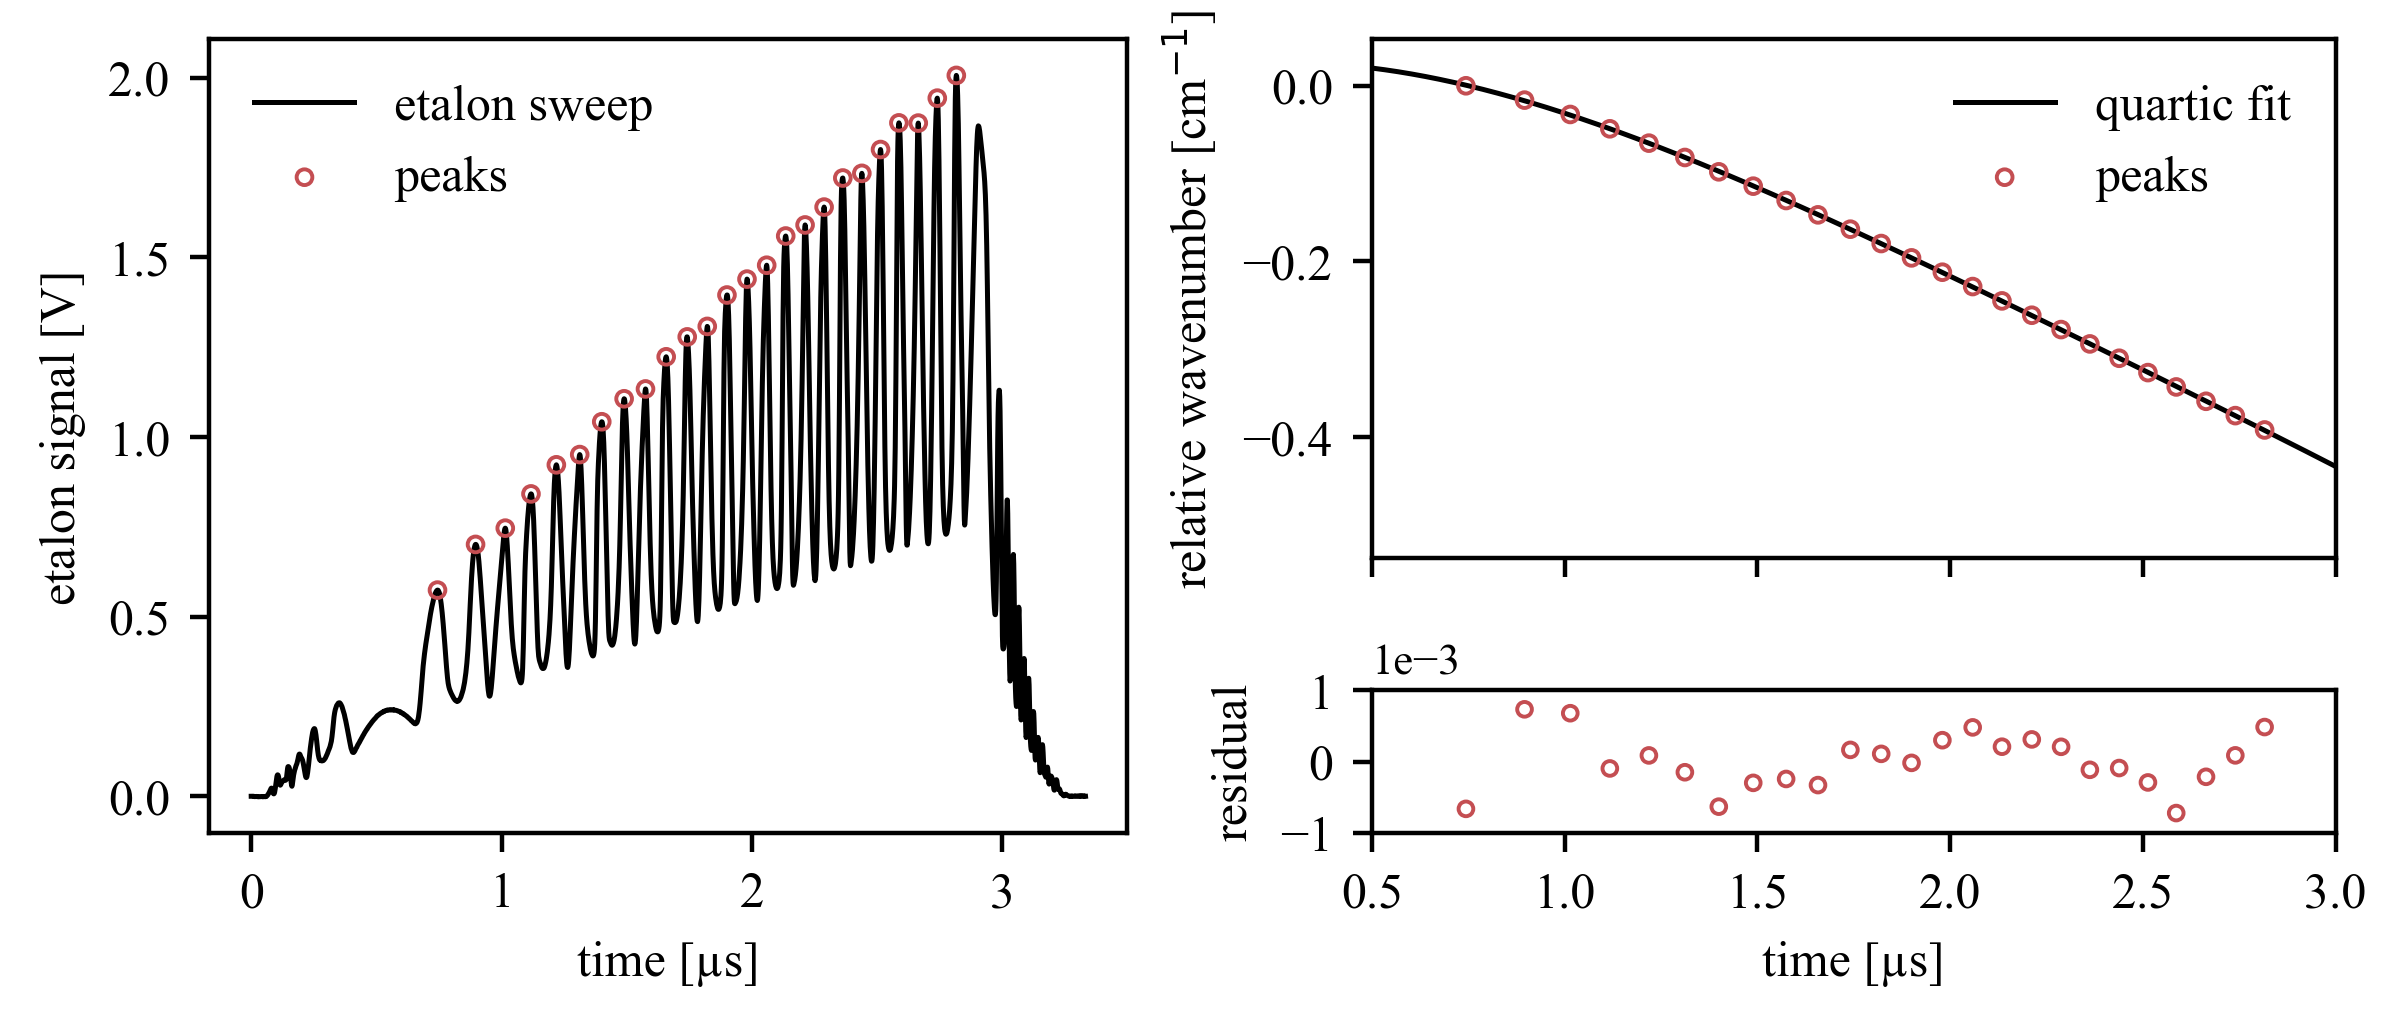
\includegraphics[width=\linewidth]{figures/etalon.png}
  \caption{Etalon-based relative wavenumber calibration. Left: representative corrected etalon sweep with detected fringe peaks. Right: quartic time-to-wavenumber fit and peak residuals.}
  \label{fig:etalon-cal}
\end{figure}

The absorbance spectrum on the calibrated frequency axis is shown together with the Voigt-profile fit in Fig.~\ref{fig:voigt-fit}, discussed in the next section.

\section{Results and Discussion}

\subsection*{Voigt-Fit and Data Extraction}

Each usable absorbance spectrum is fit with a constrained sum of three Voigt profiles using SciPy's Voigt-profile function and nonlinear least squares. The fit is not fully free. Instead, the optimizer works on an eight-parameter vector consisting of one shared temperature, the anchor line center for P(0,31), a small center adjustment for P(2,20) relative to its nominal offset from P(0,31), one collisional half-width for P(0,31), one shared collisional half-width for P(2,20) and P(3,14), one integrated area for P(0,31), and a linear baseline offset and slope. The explicit per-line centers, widths, and areas reported after the fit are reconstructed from this reduced parameterization.

The handout recommendations for stabilizing the fit were implemented directly. The weakest transition, P(3,14), is held at a fixed offset from the anchor line P(0,31), and P(3,14) is forced to share its collisional width with P(2,20). Additional constraints were added for the same reason. Only the strongest integrated area is fit freely; the areas of the weaker transitions are tied to it through the temperature-dependent line-strength ratios, so once the shared temperature is specified the weaker areas are no longer independent. A small linear baseline is also retained inside the spectral fit to absorb any residual broadband mismatch left after the time-domain baseline correction. These choices are mainly about stability: when all three lines are allowed to vary independently, the optimizer can swap line identities or trade area between overlapping features.

The main purpose of the fit is to extract the quantities needed for the state solve in a stable way. Temperature is taken directly from the shared Doppler term. The fitted Lorentz half-width of the strongest transition, P(0,31), is converted to collisional FWHM and used in the pressure relation, while the integrated area of that same line is used in the absorbance-area relation. Pressure and CO mole fraction are then solved simultaneously from those two quantities with temperature held fixed. The weaker transitions are therefore still important, but mainly because they stabilize the spectral decomposition and improve the temperature estimate rather than because they enter the final pressure solve directly. To improve continuity sweep-to-sweep, the previous successful fit is used as the initial guess for the next spectrum, and spectra with peak absorbance below the minimum threshold are skipped.

A representative constrained fit is shown in Fig.~\ref{fig:voigt-fit}. The measured absorbance and total model agree very closely. The dotted vertical lines mark the fitted line centers. The dominant peak is anchored by P(0,31), the lower-wavenumber feature is dominated by P(2,20), and P(3,14) appears as a weaker shoulder on the high-wavenumber side of the main peak. The residual remains small compared with the peak absorbance, which indicates that the constrained model is capturing the spectrum without obvious line swapping or baseline distortion.

\begin{figure}[tbp]
  \centering
  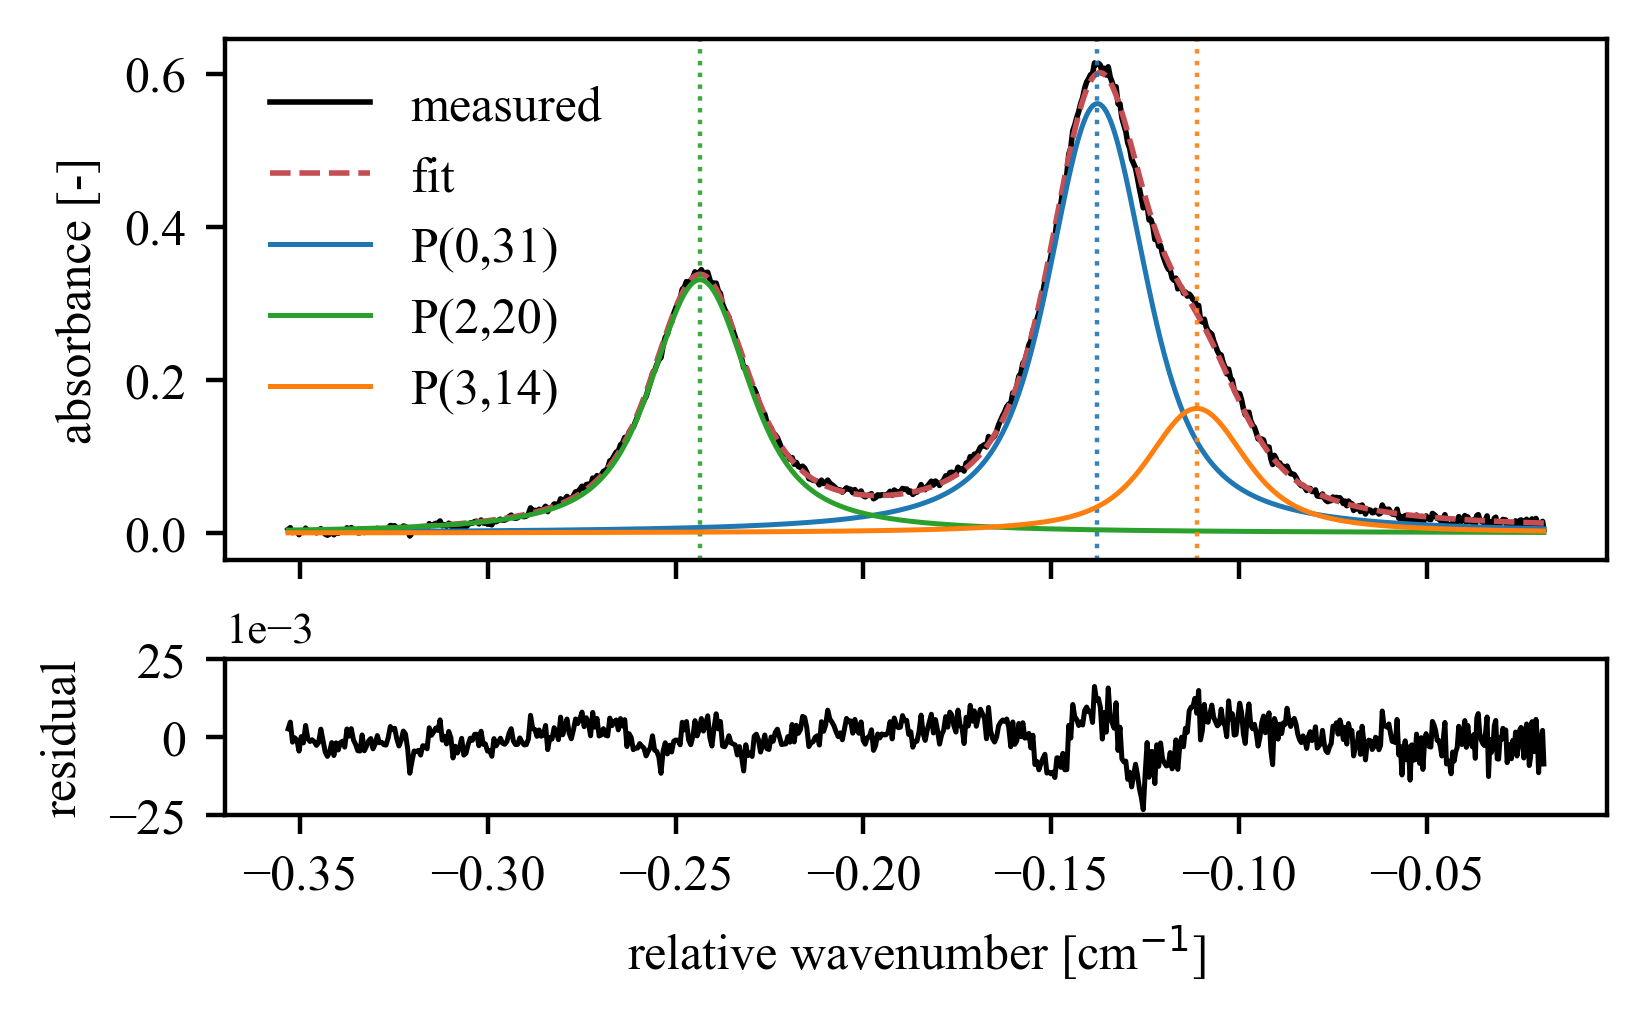
\includegraphics[width=4 in]{figures/voigt_fit.png}
  \caption{Representative constrained three-line Voigt-profile fit. The measured absorbance is shown together with the total fit, the individual transition contributions, fitted line-center markers, and the residual.}
  \label{fig:voigt-fit}
\end{figure}

\subsection*{Recovered State Histories}

The recovered temperature, pressure, and CO mole-fraction histories are shown in Fig.~\ref{fig:state-history}. The first few points, up to about \SI{50}{\micro\second}, correspond to Region~2 of the shock tube: behind the incident shock but before arrival of the reflected shock. That interval is short, so the state is only weakly constrained by the available scans, but the recovered CO mole fraction near \num{0.02} is consistent with the initial driven-gas composition.

At about \SI{50}{\micro\second}, the reflected shock reaches the test section and the recovered state moves into Region~5. The pressure jumps abruptly to nearly \SI{1}{atm}, and the temperature rises at the same time to about \SI{4000}{K}, matching the nominal target condition. The CO mole fraction increases more gradually, then levels off just below 4\%, which is broadly consistent with the initial mixture if most of the \ce{CO2} dissociates to \ce{CO} under the reflected-shock conditions.

That Region~5 state remains approximately steady for about \SI{350}{\micro\second}. After that, the pressure rises while the temperature falls, and the recovered CO mole fraction also decreases. Based on the measured state history, that late-time behavior is consistent with both recombination toward \ce{CO2} and dilution by driver gas. Because this interpretation is based only on the laser-absorption data, the late-time evolution should still be treated more cautiously than the initial reflected-shock plateau.

The uncertainty bands are included in Fig.~\ref{fig:state-history} to show where the recovered state is tightly or weakly constrained. They remain relatively narrow through much of the early and mid-time record and then widen toward the end as the spectra weaken and the fitted pressure becomes more sensitive to linewidth uncertainty. A full description of how those uncertainty bands were constructed is included in the next section.

\begin{figure}[tbp]
  \centering
  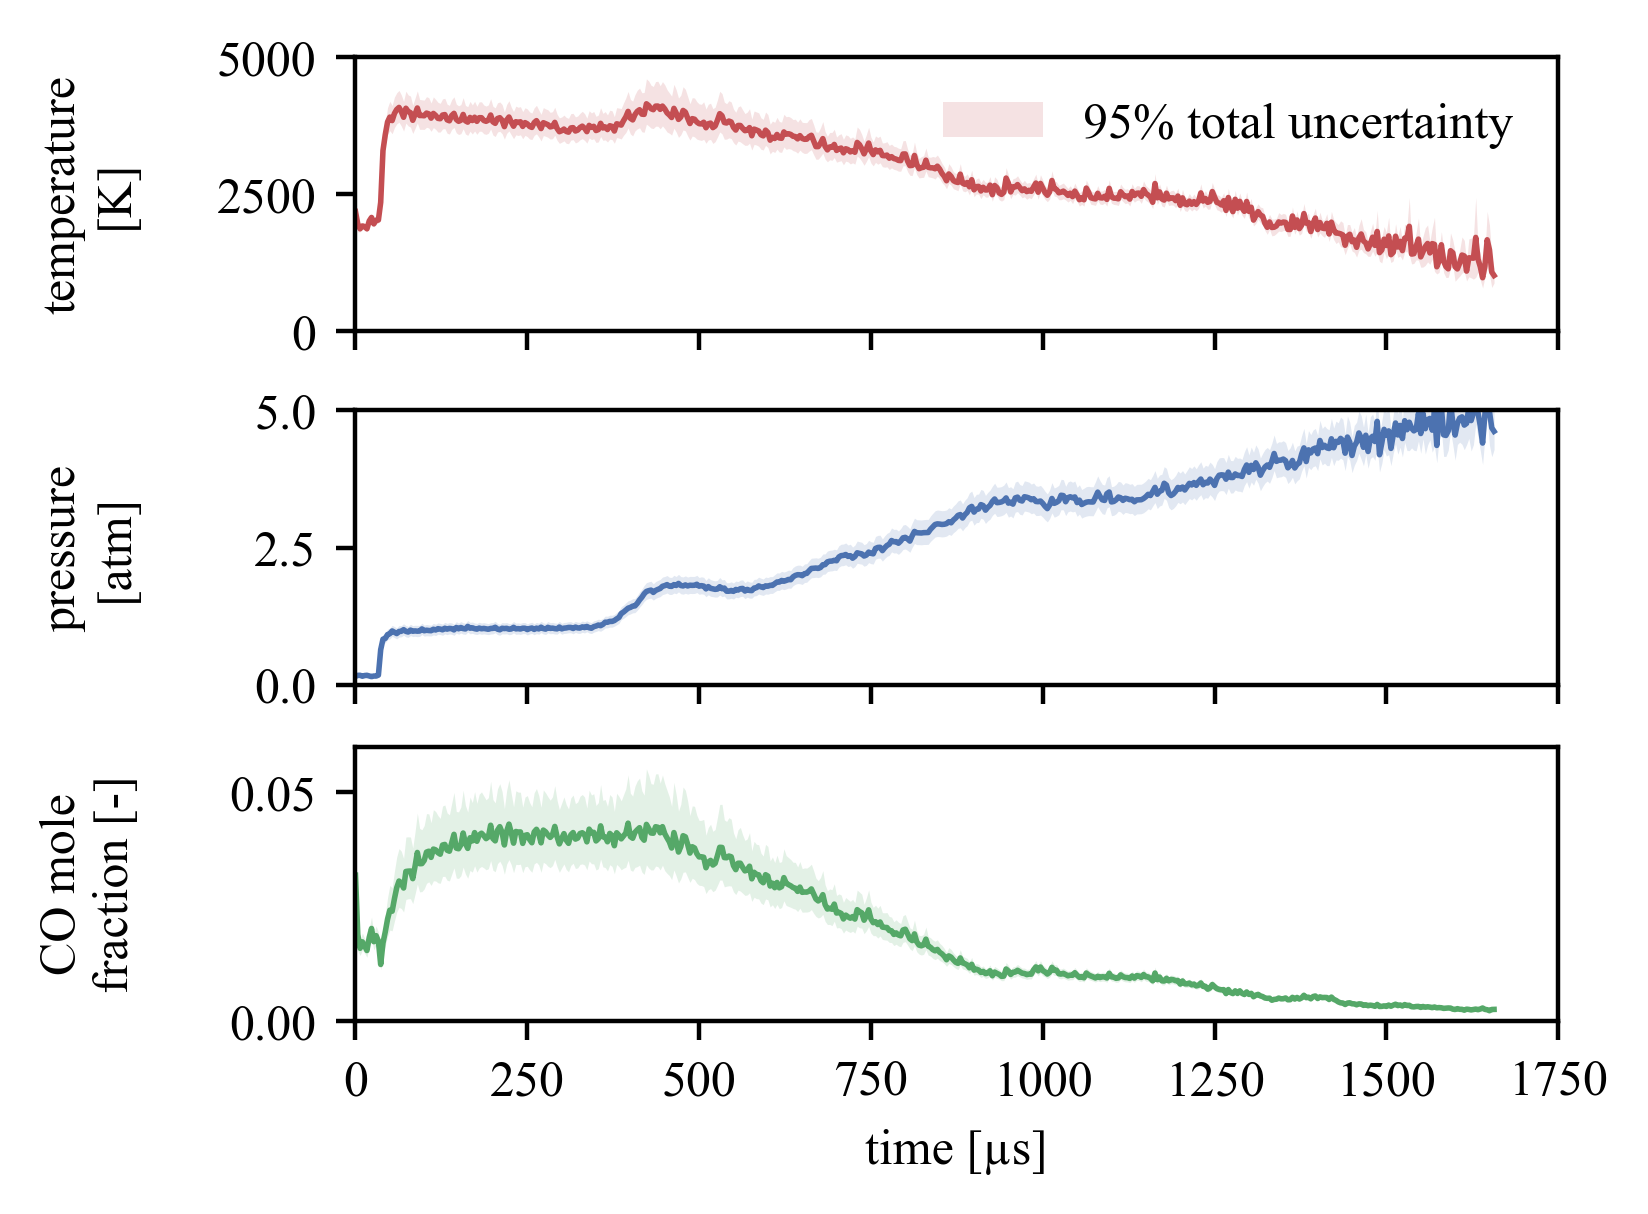
\includegraphics[width=4 in]{figures/state_history.png}
  \caption{Recovered temperature, pressure, and CO mole-fraction histories. The shaded bands show the total 95\% uncertainty carried forward to the reported state variables; the uncertainty model itself is discussed in the next section.}
  \label{fig:state-history}
\end{figure}

\section{Uncertainty}

\subsection*{Fit and Spectroscopic Contributions}

Two independent uncertainty sources were carried through the analysis. The first is local fit uncertainty from the constrained nonlinear least-squares problem. That contribution is estimated from the fit Jacobian, which gives a local covariance for the reduced fit parameters under the usual linearization of the model near the optimum. The covariance is then propagated through the parameter expansion and state-extraction steps to obtain uncertainty in temperature, pressure, and CO mole fraction.

The second source is uncertainty in the spectroscopic inputs. That contribution was treated with a full Monte Carlo refit of the data using jittered spectroscopic parameters. For each of 1000 trials, the sampled parameters were drawn uniformly within the bounds implied by the HiTEMP/HITRAN uncertainty data, consistent with NIST Technical Note 1297, and the full constrained Voigt-fit and state-solve workflow was repeated.

The two uncertainty sources were treated as linearly independent and combined by root-sum-square of their 95\% half-widths. The resulting total uncertainty is included in Fig.~\ref{fig:state-history}. In the Region~5 data, the combined uncertainty is dominated by the spectroscopic contribution, while at late time the weakening spectra make the fit uncertainty the larger term.

\section{Conclusions}

The provided scans were reduced to baseline-corrected absorbance spectra, calibrated on a relative frequency axis with the etalon, fit with a constrained three-line Voigt model, and converted into time-resolved estimates of temperature, pressure, and CO mole fraction. The recovered histories identify the expected sequence of shock-tube states: an early Region~2 interval before reflected-shock arrival, followed near \SI{50}{\micro\second} by a Region~5 state close to the target condition of \SI{\sim 4000}{K} and \SI{\sim 1}{atm}. The CO mole fraction rises more gradually than the thermodynamic variables and then levels off just below 4\%, which is broadly consistent with substantial \ce{CO2} dissociation under the reflected-shock condition.

The main limitations are the modeling assumptions required to make the reduction stable from the available absorption data alone. Pressure extraction treats all non-CO collisions as a single nitrogen-equivalent bath gas and applies the suggested fixed 0.84 scaling factor, neither of which is a fully species-resolved reacting-mixture broadening model. The frequency calibration is relative rather than absolute, and the spectral fit also constrains the weakest transition by fixing its offset from the anchor line and forcing it to share a collisional width with the secondary line. Those choices are reasonable for stability, but they likely reduce absolute accuracy when the real line positions or broadening behavior depart from the constrained model.

If the measurement were repeated, the two changes most likely to improve accuracy would be an absolute frequency reference and a better broadening model for the reacting mixture. Additional benefit would likely come from stronger independent constraint on the weak transitions, either through improved signal-to-noise or by selecting a scan window with better line separation.

\section*{References}

\begin{enumerate}
  \item G. C. Mathews, M. G. Blaisdell, A. I. Lemcherfi, C. D. Slabaugh, and C. S. Goldenstein, ``High-bandwidth absorption-spectroscopy measurements of temperature, pressure, CO, and H$_2$O in the annulus of a rotating detonation rocket engine,'' \textit{Applied Physics B}, 2021. doi:10.1007/s00340-021-07703-9.
\end{enumerate}

\end{document}
